\section{Assessing search spaces of GenProg and SPR}

In this section, we describe the empirical study, in which we manually examined \numvuln Android vulnerabilities to assess the effectiveness of GenProg and SPR search spaces, and present the results.

\subsection{Methodology}

% Purpose
During this empirical study, we aimed to answer the following research question: how effective are the search spaces of GenProg and SPR in fixing Android vulnerabilities?
To answer it, we manually examined developer fixes for \numvuln previously mined vulnerabilities, and for each we made a decision whether the developer fix is in the search space of a particular tool.

% Search spaces
Section~\ref{section:background} provides information on how GenProg and SPR search spaces are structured; to conduct such an empirical study, a precise understanding of the GenProg and SPR search spaces is needed (e.g., what are the ingredients for GenProg? What types of variables can be used by SPR?). Before commencing the study, the authors of this work thoroughly discussed what each tool can and cannot do; during the manual examination, the authors discussed between each other particularly unclear cases.

% website
To facilitate the process of manual examination, we created a service in the form of a website that allows to go through all the vulnerabilities and make a decision for each.
Figure~\ref{figure:website-main} shows the main page of the website that lists all the vulnerabilities.
By clicking on a vulnerability, a vulnerability (using the ASB terminology, cf. Section~\ref{section:mining-acquiring}) description open (Figure~\ref{figure:website-vuln}); it also allows to go to the next of the previous vulnerability.
A vulnerability page contains a list of associated CVEs; by clicking on a CVE link, a CVE-description page opens (Figure~\ref{figure:website-cve}).
This page also contains the developer patch that fixes this CVE; the patch is presented by pulling the \texttt{git diff} information from a corresponding git-repository.
To assess the GenProg search space, an ingredient search can be conducted by putting a particular statement into the search bar (cf. Figure~\ref{figure:website-marking}).
After the decision is made, corresponding check-marks are manually set and the database is updated.

% release
We release the source code and deployment instructions for the presented service\footnote{https://github.com/last5bits/cs858/tree/master/MarkWebsite}.
These materials should be helpful not only for the purposes of reproducing our study, but also for conducting similar studies or extending the current one.

\begin{figure}[t!]

\begin{subfigure}[b]{\linewidth}
    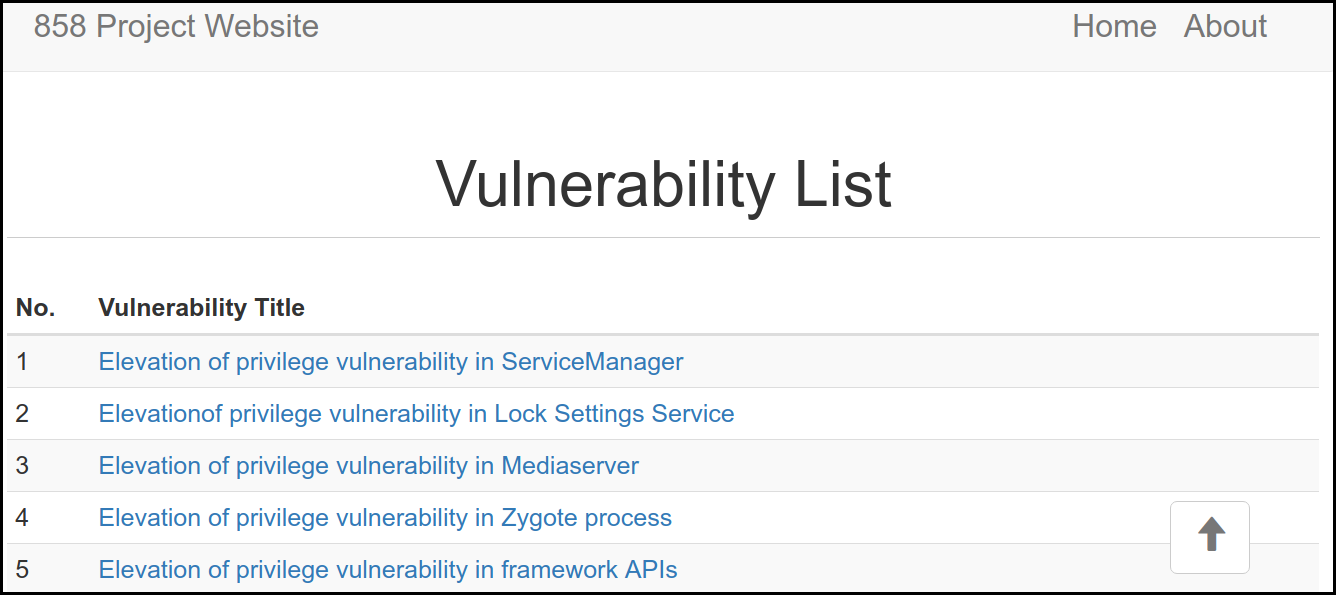
\includegraphics[width=\linewidth]{website-main}
    \caption{Main page}
    \label{figure:website-main}
\end{subfigure}

\begin{subfigure}[b]{\linewidth}
    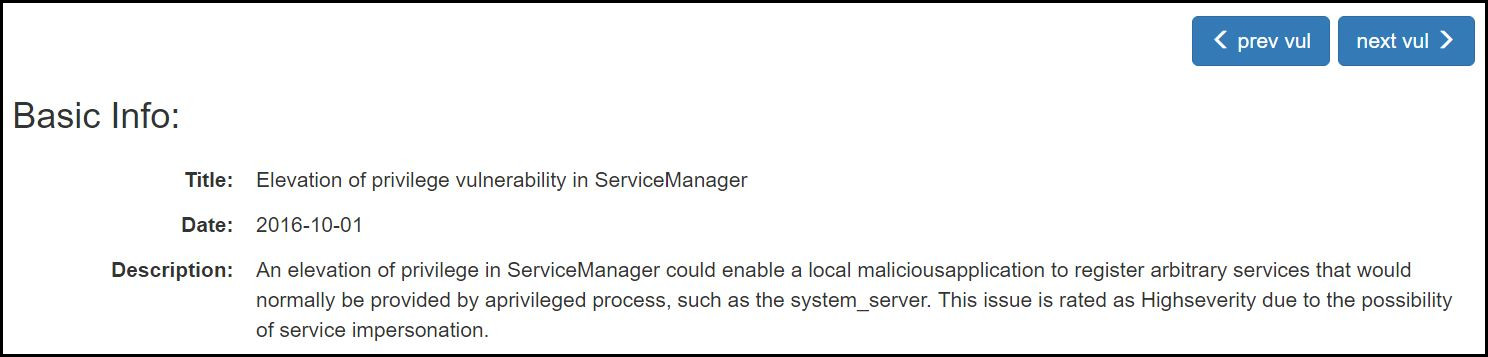
\includegraphics[width=\linewidth]{website-vuln}
    \caption{Vulnerability description}
    \label{figure:website-vuln}
\end{subfigure}

\begin{subfigure}[b]{\linewidth}
    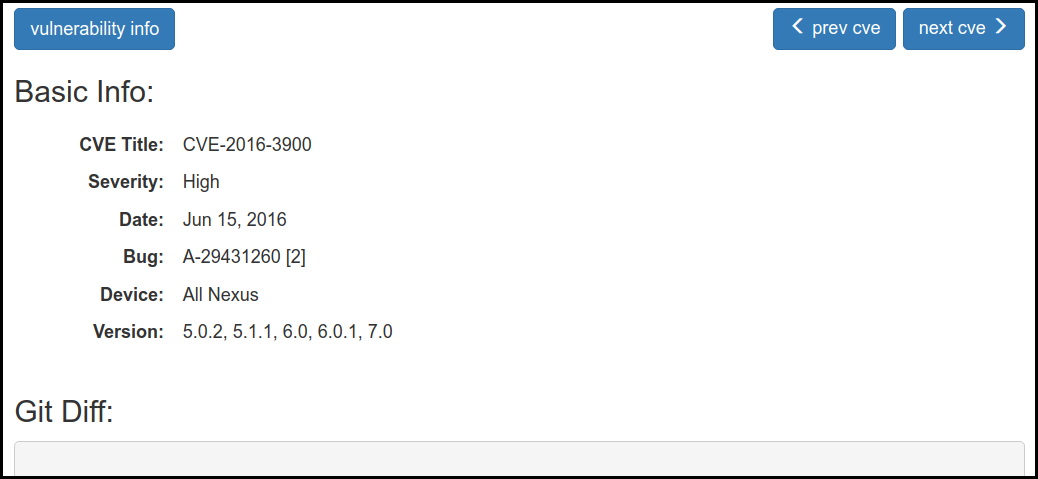
\includegraphics[width=\linewidth]{website-cve}
    \caption{CVE information}
    \label{figure:website-cve}
\end{subfigure}

\begin{subfigure}[b]{\linewidth}
    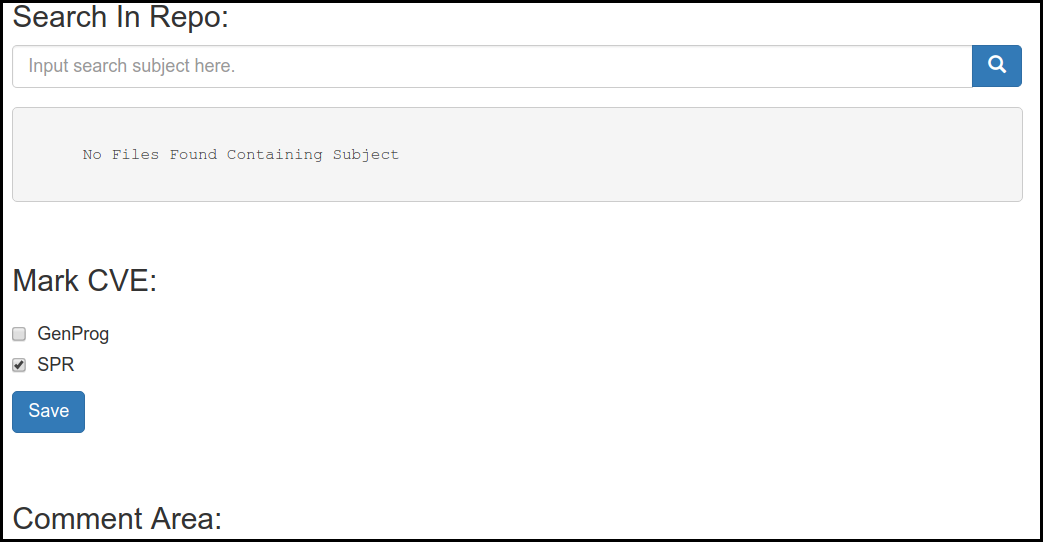
\includegraphics[width=\linewidth]{website-marking}
    \caption{Marking section}
    \label{figure:website-marking}
\end{subfigure}

\caption{A service to conduct the empirical study}
\label{figure:website}
\end{figure}

\subsection{Results of assessing the search spaces}

% Venn diagram GenProg / SPR
